%% ma: L12-B03-0016
%% lop: 12
%% chuong: 1
%% bai: 3
%% dang: 12.3.8
%% loai: TN4
%% muc: TH
%% dap_an: "C"
%% nguon: "(NBV)-ĐỀ SỐ 19-MỖI NGÀY 1 ĐỀ THI 2025.pdf (D19, MỖI NGÀY 1 ĐỀ - Đề số 19), Phần I Câu 2"
%% kien_thuc: "Bài 3 (tiệm cận đứng, tiệm cận ngang đọc từ bảng biến thiên)"
%% trang_thai: chinh-thuc
%% ghi_chu: "Đáp án gốc C đúng (tiệm cận ngang y = 1, y = 3; tiệm cận đứng x = 0). Trùng ý tưởng với dạng đã duyệt 12.3.8 (tổng số tiệm cận đứng và ngang từ các giới hạn), ở đây các giới hạn đọc từ bảng biến thiên; nhập chính thức."
\begin{ex}
Cho hàm số $y=f(x)$ có bảng biến thiên như sau:
\begin{center}
\begin{tikzpicture}
  \tkzTabInit[lgt=1.4,espcl=2.6]{$x$/.8,$y'$/.8,$y$/2.6}{$-\infty$,$0$,$3$,$+\infty$}
  \tkzTabLine{,-,d,-,0,+,}
  \tkzTabVar{+/$1$,-D+/$-\infty$/$+\infty$,-/$-3$,+/$3$}
\end{tikzpicture}
\end{center}
Tổng số tiệm cận đứng và tiệm cận ngang của đồ thị hàm số đã cho là
\choice{$4$}{$1$}{\True $3$}{$2$}
\loigiai{Từ bảng biến thiên: $\lim\limits_{x\to-\infty}f(x)=1$ và $\lim\limits_{x\to+\infty}f(x)=3$ nên đồ thị có hai tiệm cận ngang $y=1$, $y=3$. Vì $\lim\limits_{x\to0^-}f(x)=-\infty$ và $\lim\limits_{x\to0^+}f(x)=+\infty$ nên $x=0$ là tiệm cận đứng. Tổng cộng có $3$ đường tiệm cận. Chọn C.}
\end{ex}
